\documentclass[12pt,a4paper]{article}
\usepackage{float}
\usepackage{graphicx}
\usepackage{xcolor}
\usepackage[left=2cm,right=2cm,top=2cm,bottom=2cm]{geometry}

\author{Swara Patil \\ MM22B045}
\title{Assignment 4}
\date{June 16, 2023}

\begin{document}
\maketitle

\section{MM22B045}
\subsection{Name}
Swara Sunil Patil
\subsection{GitHub User ID}
SSPIIT
\subsection{Hooke's Law}
Hooke’s law states that the strain of a material is proportional to the applied stress within the elastic limit of that material~\cite{byjus}.
$$\colorbox{yellow}{$\sigma \propto \epsilon$}$$
where,\\
$\sigma$ is the tensile stress and \\
$\epsilon$ is the strain~\cite{wiki}.\\ 
We can express this relationship with a proportionality constant as follows:
$$\sigma = E\epsilon$$
$E$ is called the modulus of elasticity.\\ Equation~\ref{eq1} shows the relationship between force, area, and change in length:
\begin{equation}
    \frac{F}{A} = E\frac{\Delta L}{L}
    \label{eq1}
\end{equation}
Since, $$\sigma = \frac{F}{A}$$\\
represents the stress,\\ $F$ is the applied force, and \\$A$ is the area of cross-section. Similarly, $$\epsilon = \frac{\Delta L}{L}$$
represents the strain, \\where,\\
$\Delta L$ is the change in length and \\
$L$ is the original length.\\
From Equation~\ref{eq1}, we can derive the formula for change in length as:
$$\Delta L = \frac{F L}{A E}$$
Hooke's Law is applicable within the proportionality limit, as shown in Figure~\ref{erfplot}.

\begin{figure}[H]
    \centering
    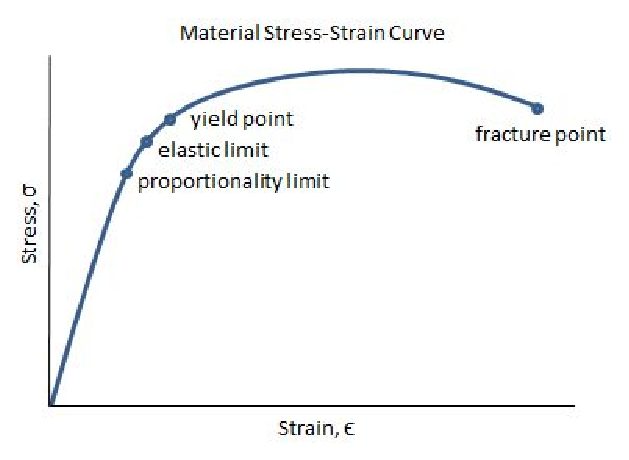
\includegraphics{hooke.eps}
    \caption{A plot of Stress vs Strain}
    \label{erfplot}
\end{figure}

\subsection{Why did I choose Hooke's Law?}
I chose Hooke's Law because it is a fundamental equation in the field of Metallurgical and Materials Engineering, which is my parent department. As a discipline that focuses on materials and their properties, stress and strain are key mechanical properties that we study. Hooke's Law provides a clear relationship between these two properties and introduces the concept of elasticity, which is crucial in understanding material behavior. I have been exposed to Hooke's Law since my high school education, and it was further reinforced in my introductory course on MM1001.

\bibliography{references}
\bibliographystyle{alpha}
\end{document}
